\documentclass[12pt]{article}
\usepackage{ucs}
\usepackage[utf8x]{inputenc}
\usepackage[turkish]{babel}
\usepackage{graphicx}
\usepackage{url}
\usepackage[sc]{mathpazo}
\linespread{1.05}
\usepackage[T1]{fontenc}
\usepackage[a2paper,margin=1cm]{geometry}
\usepackage{shapepar}
\pagestyle{empty}

\author{Mehmet Atakan Gürkan}
\title{}
\date{}
\newcommand\almleftshape{
   {0}
   {0}b{0}
\\ {0}t{0}{7}
\\ {17}t{0}{11.5}
\\ {19}t{0}{11.7}
\\ {21}t{0}{11.7}
\\ {24}t{0}{11.3}
\\ {34}t{0}{8.3}
\\ {41}t{0}{4.4}
\\ {42}e{0}}
\newcommand\almrightshape{
   {12}
   {0}b{0}
\\ {0}t{3.2}{6.8}
\\ {1}t{4}{6}
\\ {5}t{2.6}{7.4}
\\ {10}t{1.0}{9}
\\ {15}t{-0.6}{10.6}
\\ {17}t{-1}{11.0}
\\ {19}t{-1.2}{11.2}
\\ {21}t{-1}{11.0}
\\ {27}t{0}{10.0}
\\ {41}t{3.5}{6.5}
\\ {42}e{10}}
\newcommand\almrrightshape{
   {8.5}
   {0}b{0}
\\ {0}t{4.7}{3.3}
\\ {1}t{4}{4}
\\ {5}t{2.5}{5.5}
\\ {8}t{2.1}{5.9}
\\ {9}t{2.1}{5.9}
%\\ {15}t{-0.6}{10.6}
%\\ {17}t{-1}{11.0}
%\\ {19}t{-1.2}{11.2}
%\\ {21}t{-1}{11.0}
%\\ {27}t{0}{10.0}
%\\ {41}t{3.5}{6.5}
\\ {9}e{2}}
\begin{document}
%\maketitle
\shorthandoff{=}
\centerline{\raisebox{-1in}{
\includegraphics[clip,height=2.3975in]{afl_4_1}}
     \fontsize{40pt}{40pt}\selectfont
     \quad Ankara Fen Lisesi için Gökyüzü Almanağı \quad
\raisebox{-1in}{
\includegraphics[clip,height=2.3975in]{afl_4_1}}}
\vskip -1cm
\noindent
\centerline{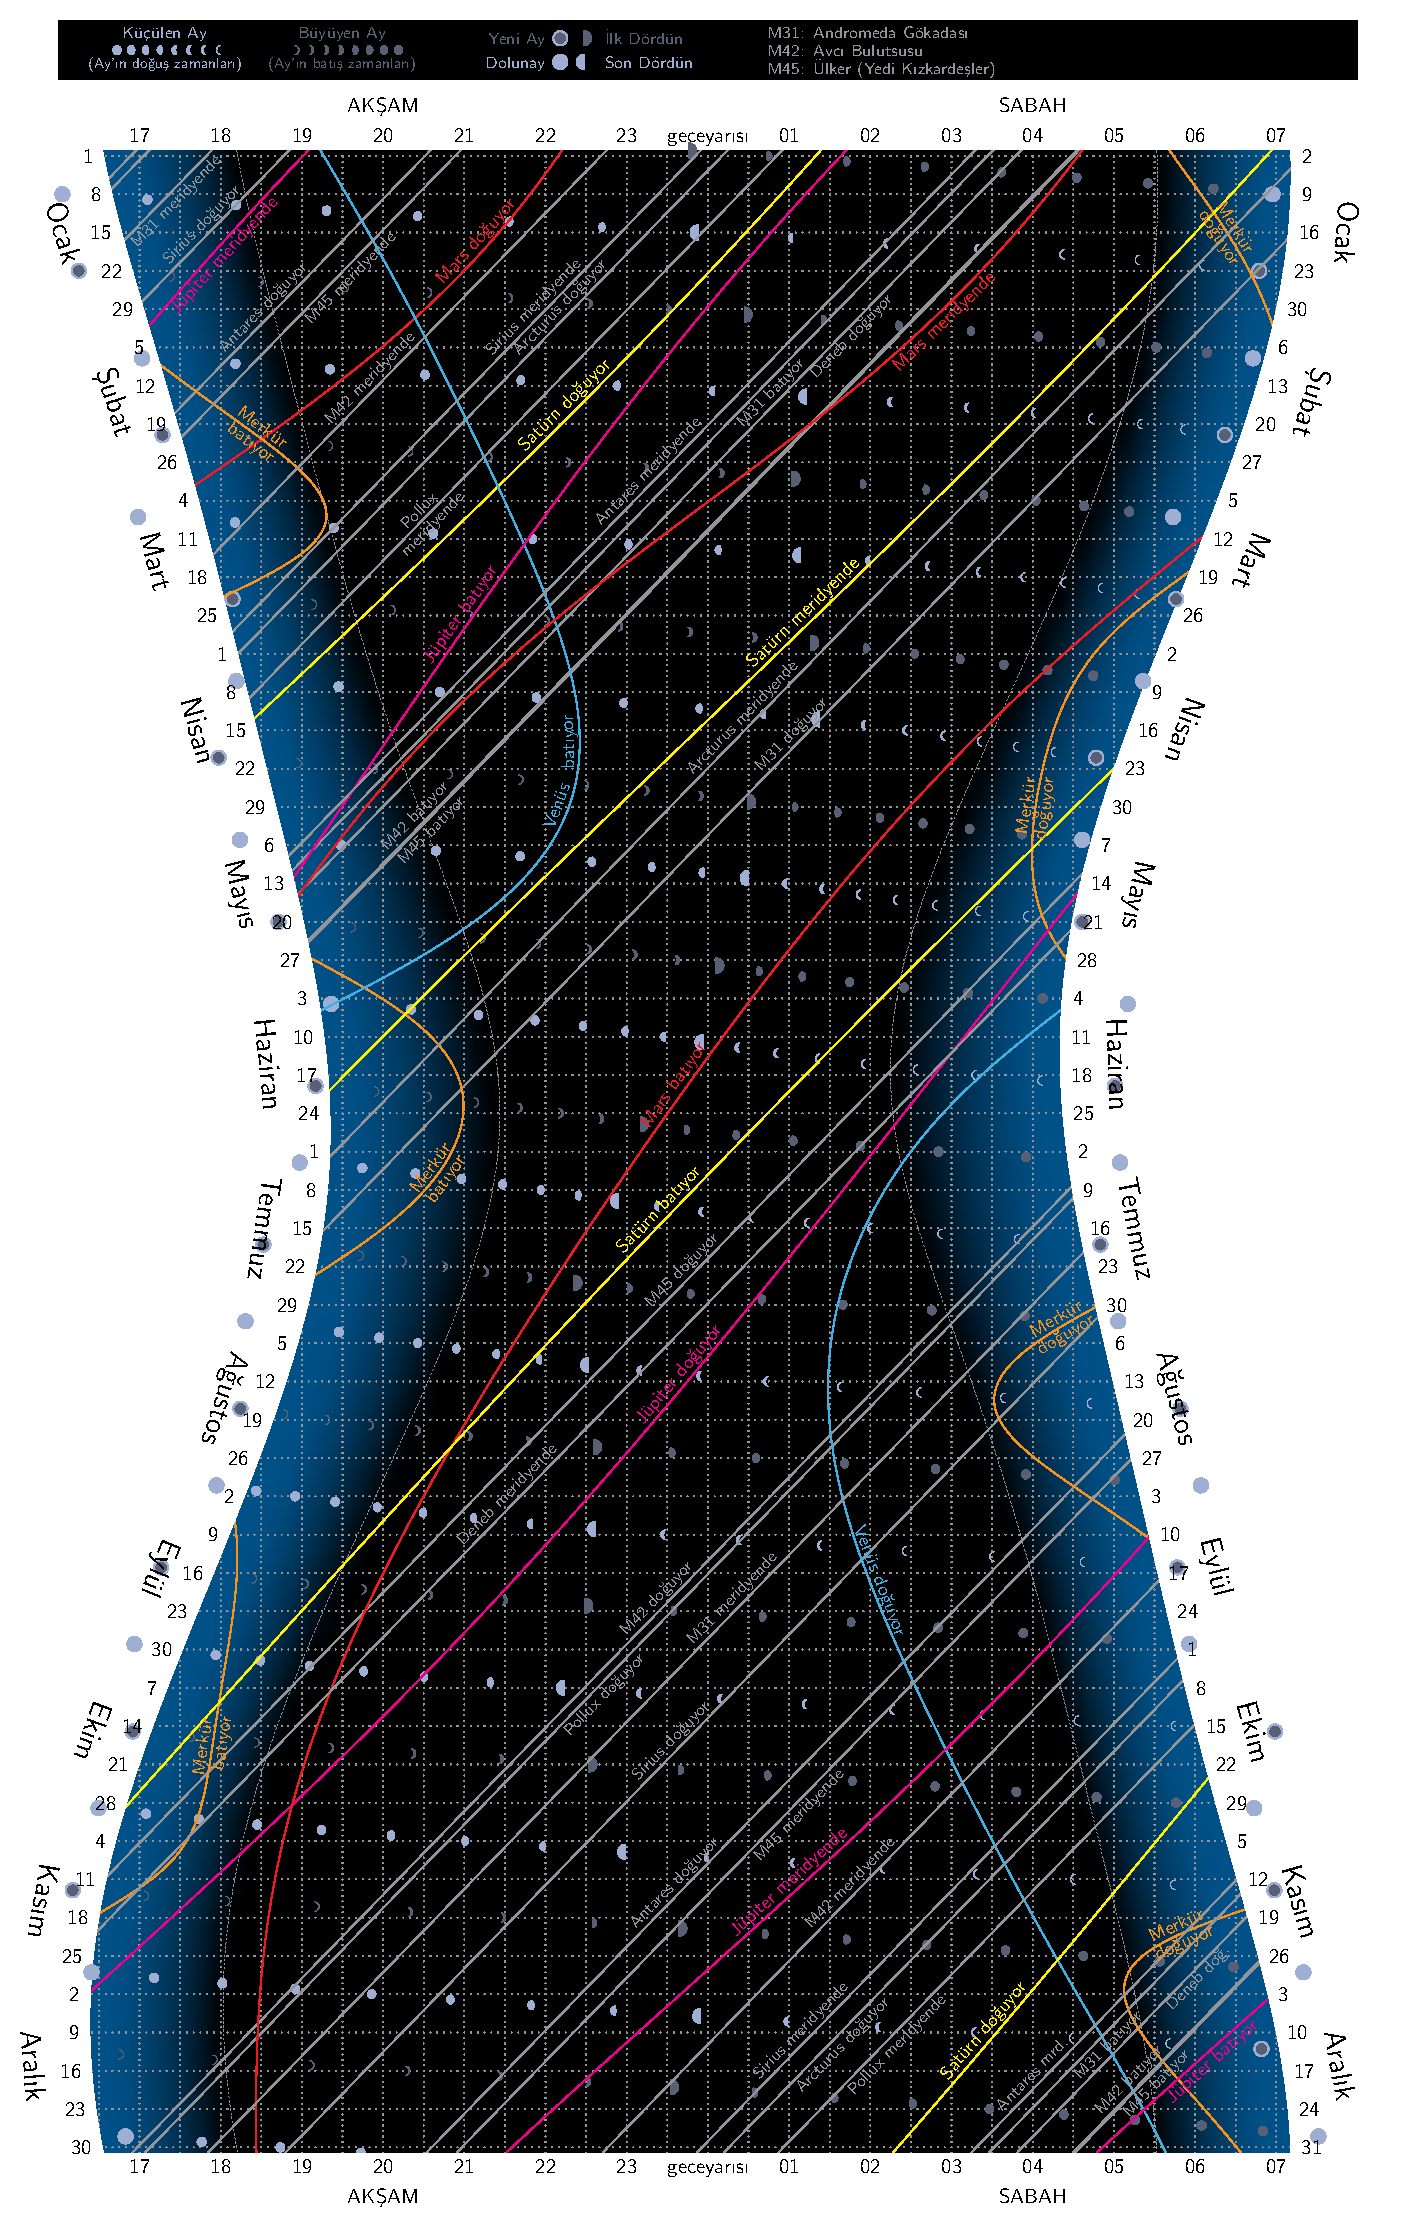
\includegraphics[clip,height=0.9\textheight]{almanac_2012_AFL}}

\vskip -0.9\textheight \vskip9.5cm
\noindent
\cutout{l}(0cm,0pt)
\shapepar{\almleftshape}{\fontsize{13pt}{13pt}\selectfont
\hskip0.4cm\textbf{Çizelgenin Kullanımı}\\
Bu çizelge 2012 yılı için, Ankara Fen Lisesi'nde çeşitli
gök cisimlerinin doğma, meridyenden (gökyüzünde ulaştıkları en
yüksek noktadan) geçme ve batma zamanlarını, alacakaranlığın
sonuyla başlangıcını ve Ay'ın evrelerini veriyor.  Dikey eksen
günleri, yatay eksen gece boyunca zamanı gösteriyor.  Gece içinde
yarımşar saatlik aralıklar ve yıl içinde Pazar akşamlarını
Pazartesi sabahlarına bağlayan geceler noktalı çizgilerle
belirtiliyor. Düşey olarak iki nokta arası bir güne, yatay olarak
iki nokta arası beş dakikaya karşılık geliyor.\\
Bir örnek olarak 9 Mart gecesinin olaylarına bakarsak: İlk olarak,
sol tarafta 11 Mart'a karşılık gelen noktanın üstünde yaklaşık
olarak 9 Mart'a karşılık gelen noktayı bulmak gerekiyor. Buradan
sağa doğru ilerlediğimizde 18:30 civarında Avcı Bulutsusu'nun
meridyenden geçeceğini görüyoruz. Bunun ardından 19:30'da
Merkür batıyor, 19:45 civarında Sirius meridyenden geçiyor ve
20:00 civarında Arcturus doğuyor. Bu bilgilerden Güneş battığı
zaman Orion Bulutsusu, Merkür ve Sirius'un ufkun üzerinde olduğunu
da anlıyoruz. Sağa doğru ilerledikçe, belli saatlerde pekçok
gökcisminin doğduğunu, meridyenden geçtiğini ve battığını
görüyoruz. 19:40 civarında gördüğümüz Ay sembolü, Ay'ın
doğuş zamanını gösteriyor ve bir sonraki gece Ay'ın daha
küçük olacağını belirtiyor. Son olarak 19:35 ve 4:50 civarında
gördüğümüz kesikli çizgiler sırasıyla alacakaranlığın
bitmesi ve başlamasını belirtiyor. Bu noktalar Güneş'in ufkun
18$^\circ$ altında kaldığı anlara karşılık geliyor.\\
Çizelgede verilen doğma ve batma zamanları, ufuk çizgisinin önünde bir engel
olmadığını varsayıyor. Eğer böyle bir engel varsa, her bir
açı derecesi yükseklik için doğma zamanı 4 dakika geç, batma zamanı da
aynı miktarda erken olacak. Benzer biçimde, yüksek bir noktadan gözlem
yapıldığı için ufuk çizgisi olması gerekenin altında ise, doğma ve batma
zamanlarının düzeltilmesi gerekecek.\\
Not: Yaz saati uygulamasının olduğu zamanlarda, çizelgedeki zamanlara
bir saat eklemek gerekiyor.}
\vskip -3.0cm
\cutout{r}(2em,6cm)
\shapepar{\almrrightshape}{\fontsize{13pt}{13pt}\selectfont
\hskip 0.6cm\textbf{Bazı Gök Olayları}\\
Bu yılın, belki de bu yüzyılın, en önemli gök olayı 6 Haziran 2012'deki
\textbf{Venüs Geçişi}. Venüs'ün Güneş'in önünden geçişi arası sekiz
yıllık çiftler halinde oluyor, bu çiftlerin arasındaki zamansa 121,5 ya
da 105,5 yıl. Bir önceki geçiş 8 Haziran 2004'teydi, bir sonraki
geçiş ise Aralık 2117'de olacak. Geçiş TSİ 01:10'da başlayacak, bu
sırada Güneş ufkun altında olacak, geçiş Güneş doğduktan sonra TSİ
7:50'de bitecek. (Gerekli önlemleri almadan Güneş'e
kesinlikle bakmayınız! Bunun nasıl yapılacağı ile ilgili bilgiyi şu
adreste bulabilirsiniz:\\
\url{http://www.tug.tubitak.gov.tr/tutulma/turkish/guvenli_gunes_gozlemi/guvenli_gunes_gozlemi.html})\\
Bu yılın sonlarına doğru, 28 Kasım 2012'de bir \textbf{Parçalı Ay
Tutulması} göreceğiz. Bu tutulma TSİ 14:15-18:51 arasında olacak.
Ülkemizde Ay doğarken tutulma önceden başlamış olacak.}

\vskip20cm\hskip32cm
\parbox{7.3cm}{\textbf{Göktaşı Yağmurları}\\
Quadrantid (Dörtlük): 3-4 Ocak\\
Lyrid (Lir): 22-23 Nisan\\
Eta Aquarid (Eta Kova): 4-5 Mayıs\\
Delta Aq. (Delta Kova): 27-28 Temmuz\\
Perseid (Perse): 12-13 Ağustos\\
Orionid (Avcı): 20-21 Ekim\\
Leonid (Aslan): 17-18 Kasım\\
Geminid (İkizler): 13-14 Aralık\\
Verilen tarihler yağmurların en yoğun olduğu zamanlardır, bunların bir
kaç gün öncesi ve sonrasında da normalden çok sayıda göktaşı
gözlenebilir.}

\vskip 17.3cm \footnotesize
{Hazırlayan: M. Atakan Gürkan ('92) \quad \url{https://github.com/atakan/PySkyAlmanac/tree/master/AFL} Gök olayları ve göktaşı yağmurları hakkındaki bilgiler Alp Akoğlu ve
Tuncay Özışık tarafından hazırlanan 2012 Gök Olayları Yıllığı'ndan
alınmıştır.}
\end{document}
